\section{Conclusion}

\subsection{Conclusion}
\begin{frame}
  \frametitle{Conclusion}
  \begin{block}{In 3 years, IPM prototype have been built, tested and reviewed.}
    \begin{itemize}
      \item The feasibility was focussed:
            \begin{itemize}
              \item Enough primary signal for profile reconstruction
              \item Field uniformity can be corrected and space charge effect is limited if ions are used
            \end{itemize}
      \item Main concern were about the readout system
            \begin{itemize}
              \item Strips may not have sufficient sensitivity
              \item MCP are sensitive to ageing
              \item Silicon detectors rise too many uncertainties
            \end{itemize}
      \item So prototypes have been tested on real beam conditions.
            \begin{itemize}
              \item At IPHI: a 3 MeV high intensity proton linac
              \item Lower energy, but flexible beam conditions
            \end{itemize}
      \item Both IPMs work but MCP is the preferred solution since:
            \begin{itemize}
              \item Bare strips may not have sufficient sensitivity
              \item Silicon detectors rise too many uncertainties
            \end{itemize}
      \item The project has been reviewed by ESS and is now in production phase.
    \end{itemize}
  \end{block}

\end{frame}

\subsection{Outlooks}

\begin{frame}
  \frametitle{Outlooks}
  \begin{block}{Background information}
    What happens if a "lost proton" hits MCP or structures around? $\implies$ simulations:
    \begin{itemize}
      \item Realistic geometry $\rightarrow$ CAD import
      \item Information about particles $\rightarrow$ not provided on time by ESS.
    \end{itemize}
  \end{block}
  \begin{columns}[T]
    \begin{column}{0.45\textwidth}
      \begin{block}{Simulation with Geant4 10.X}
        Features:
        \begin{itemize}
          \item STL import
          \item MT + MPI features
          \item SD + ROOT output
        \end{itemize}
        To do:
        \begin{itemize}
          \item Keep the geometry up to date
          \item I/O with ESS particle files.
        \end{itemize}
      \end{block}
    \end{column}
    \begin{column}{0.45\textwidth}
      Example with a dummy $2\,\mathrm{GeV}$ proton hitting an IPM frame:
      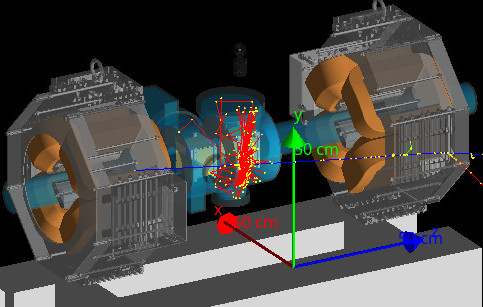
\includegraphics[width=1\textwidth]{05_Conclusion/fig/fig000_G4ESS2}
    \end{column}
  \end{columns}
\end{frame}

\begin{frame}
  \frametitle{Outlooks}
  \begin{columns}[T]
    \begin{column}{0.45\textwidth}
      \begin{block}{Calibration}
        A MCP is subject to ageing: the gain decrease over time.
        \begin{itemize}
          \item An uniform VUV ($<200\,\mathrm{nm}$) light irradiate the MCP input surface
          \item The MCP response is recorded by camera revelling non uniform area.
          \item The new calibration map is applied on beam images.
        \end{itemize}
      \end{block}
    \end{column}
    \begin{column}{0.45\textwidth}
      \begin{center}
        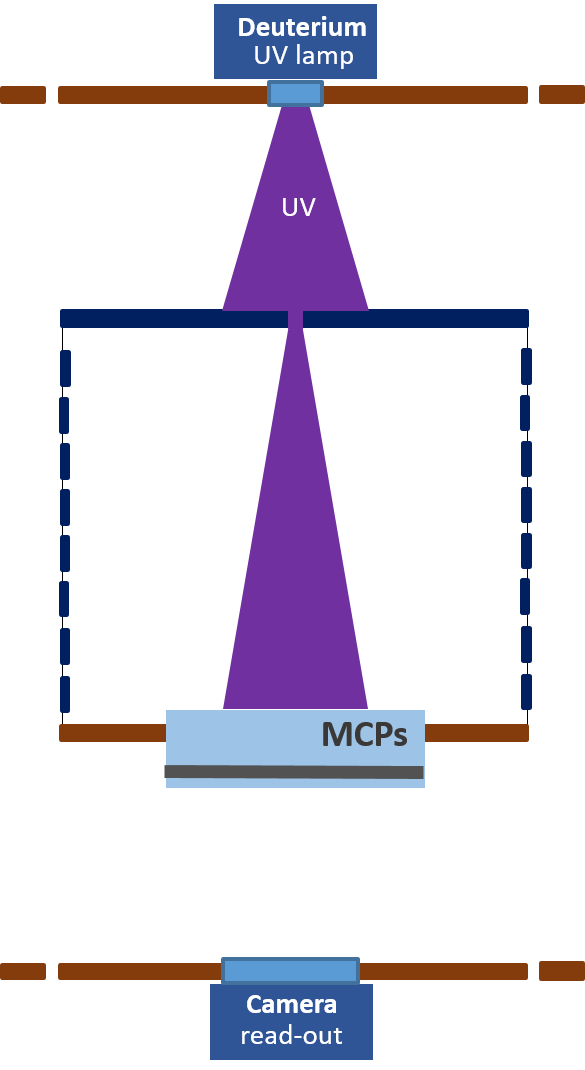
\includegraphics[width=0.5\textwidth]{05_Conclusion/fig/fig000_UV_calib}
      \end{center}
    \end{column}
  \end{columns}
  \begin{columns}[T]
    \begin{column}{0.60\textwidth}
      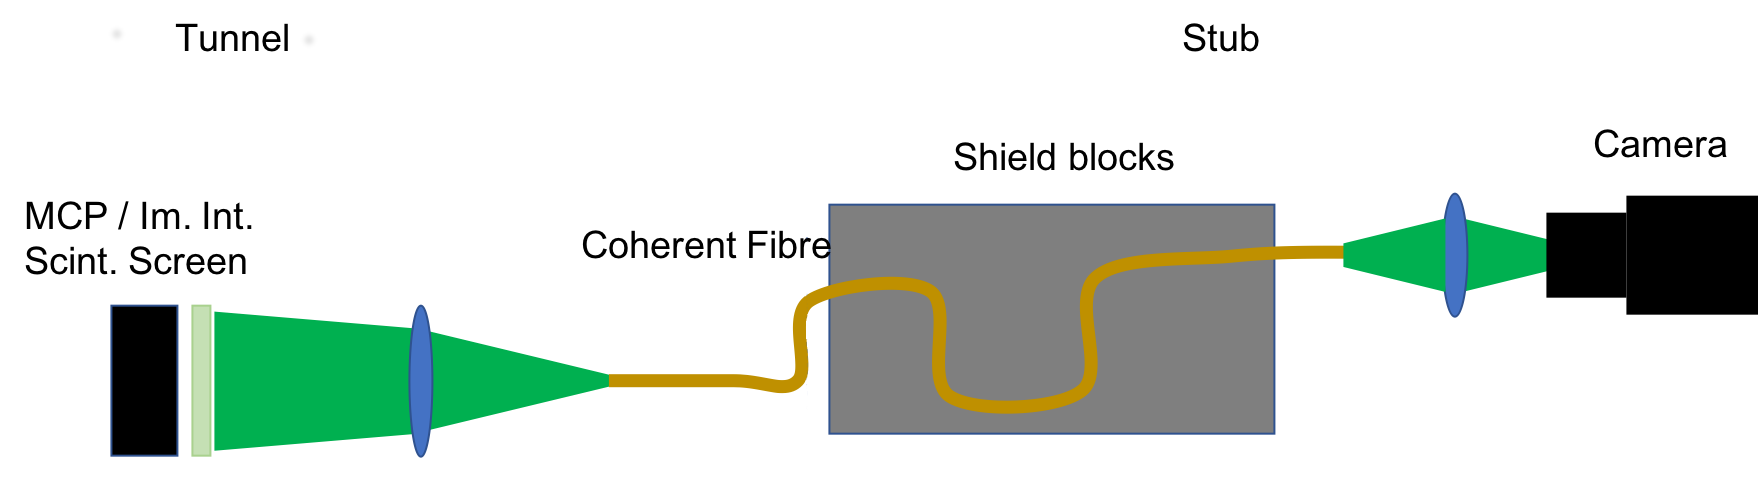
\includegraphics[width=1\textwidth]{05_Conclusion/fig/fig000_schematic_coherentr_fiber}
    \end{column}
    \begin{column}{0.35\textwidth}
      \begin{block}{Remote acquisition}
        \begin{itemize}
          \item[+] Move camera away
          \item[-] Signal and resolution decreased
        \end{itemize}
      \end{block}
    \end{column}
  \end{columns}
\end{frame}

\begin{frame}
  \frametitle{Outlooks}
  \begin{columns}[T]
    \begin{column}{0.45\textwidth}
      \begin{block}{Improved design for MCP usage}
        \begin{itemize}
          \item CF200 sustains the IPM cage, should not be moved.
          \item CF160 sustains the MCP systems for replacement.
        \end{itemize}
      \end{block}
      \begin{block}{Production}
        \begin{itemize}
          \item Compliant with superconducting cavities.
          \item Production in ISO5 cleanroom
          \item Close collaboration with the IRFU cryomodule team
        \end{itemize}
      \end{block}
    \end{column}
    \begin{column}{0.45\textwidth}
      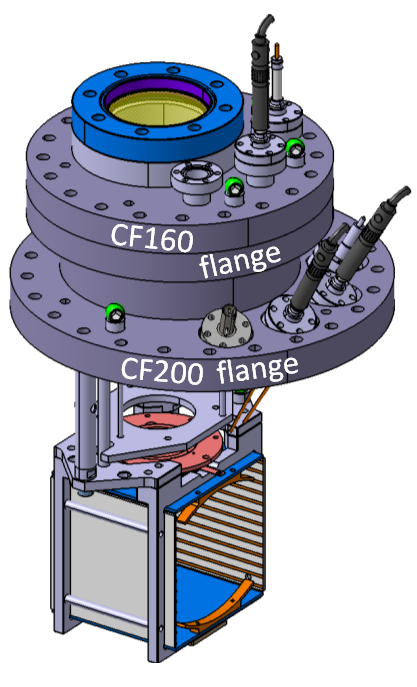
\includegraphics[width=0.75\textwidth]{05_Conclusion/fig/fig000_bride_double2_a}
    \end{column}
  \end{columns}
\end{frame}

\begin{frame}
  \frametitle{Beyond ESS}
  \begin{columns}[T]
    \begin{column}{0.45\textwidth}

    \end{column}
    \begin{column}{0.45\textwidth}
      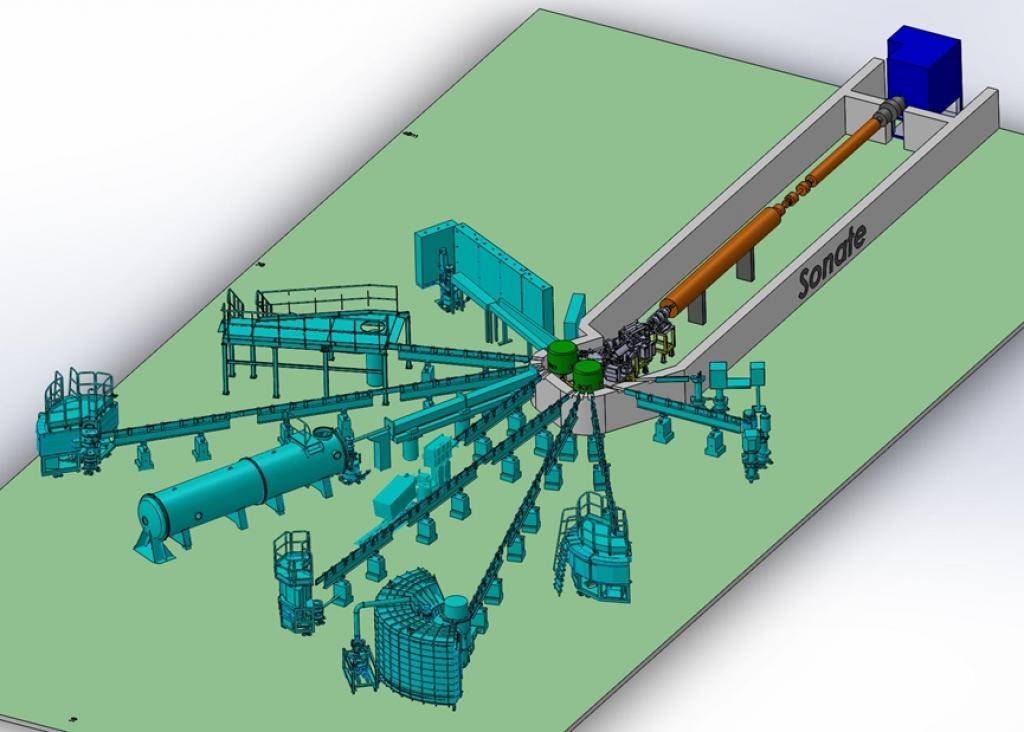
\includegraphics[width=1\textwidth]{05_Conclusion/fig/fig000_SONATE}
    \end{column}
  \end{columns}
\end{frame}